\subsection{Inlet Sweep Angle, Offset Angle, and AoA Limit - Melanie Grande}
The first parameter sweep became necessary following the  development from the inlet and maneuver controller designs. As explained in the inlet simulation section, the air influx across the inlet area experiences mass flow and pressure losses at angles of attack. In order to limit these losses, the implementation of a maximum AoA became necessary. This AoA limit would need to consider the typical orientation of the SFRJ stage at cruise and during the maneuvers, as well as the impact of the losses on the operability of the combustion chamber. A trade study was a natural solution to finding the limit that would allow maximized ground range.

This parameter sweep also included other variables related to the inlet design, such as sweep angle and offset angle, or "droop". The ideal design would facilitate optimal conditions during flight and maximize ground range. The results are presented in Figs. \ref{fig:aoaVsSweep} and \ref{fig:aoaVsOffset}. 

\begin{figure}[H]
    \centering
    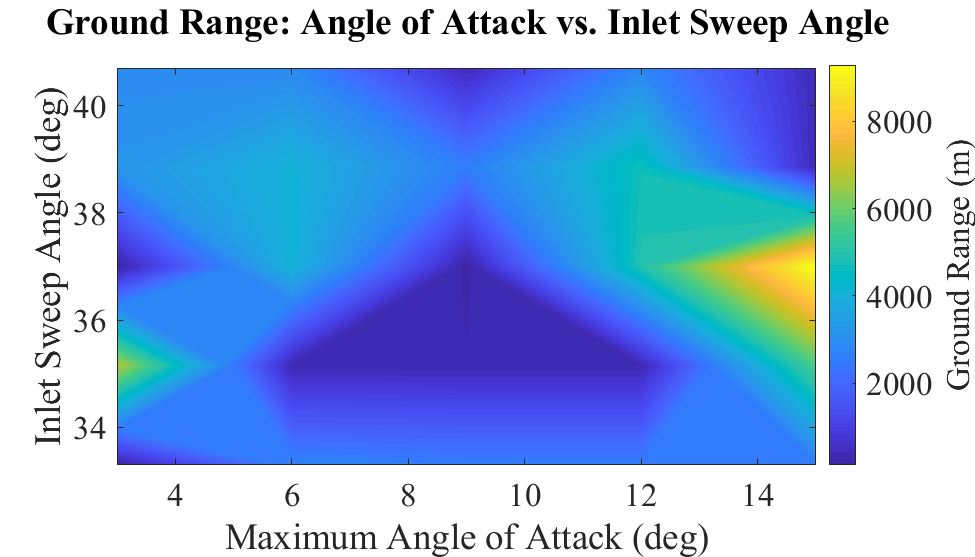
\includegraphics[width=0.7\textwidth]{ParameterSweeps/figures/RangevsAoAvsSweep.png}
    \caption{Caption}
    \label{fig:aoaVsSweep}
\end{figure}

\begin{figure}[H]
    \centering
    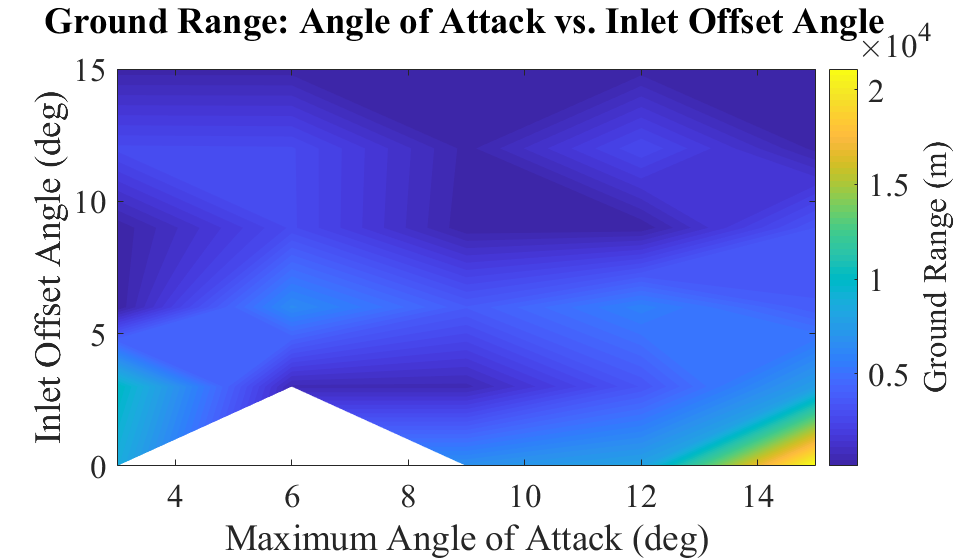
\includegraphics[width=0.7\textwidth]{ParameterSweeps/figures/RangevsAoAvsOffset.png}
    \caption{Ground range results from trading angle of attack limit and inlet sweep angle.}
    \label{fig:aoaVsOffset}
\end{figure}

Target regions were identified from each set of results to inform the evolved baseline design. From Fig. \ref{fig:aoaVsSweep}, we can see that ground range is maximized in a few different regions, and the target region selected was at an AoA limit from 10-12\textdegree and a sweep angle from 37-38\textdegree. Although there are two small triangles where the range appears to spike, further analysis of the data made the design team consider these as failures in the run using that combination, including inlet unstarting or other anomalies, so these regions were not considered. Other parameter sweeps, discussed in following sections, reflect such run failures as well.

Analysis of the ground range results for AoA limit versus droop angle revealed that the droop did not improve the SFRJ performance as the team had hoped. Perhaps a 1-5\textdegree droop could have a positive effect on the achieved ground range; however, the team chose a baseline design with zero droop. 